\documentclass[12pt]{article}
\usepackage{parskip}
\usepackage[letterpaper, margin=1in]{geometry}
\usepackage{graphicx}
\usepackage{subcaption}
\usepackage{amsmath}
\graphicspath{{./images/}}
\title{ELECENG 2EI5 Lab 4}
\author{Raeed Hassan \\ hassam41 \\  \\ McMaster University}
\begin{document}
\maketitle
\pagebreak

\begin{enumerate}
    \item The photograph of the hardware setup.
    \begin{center}
        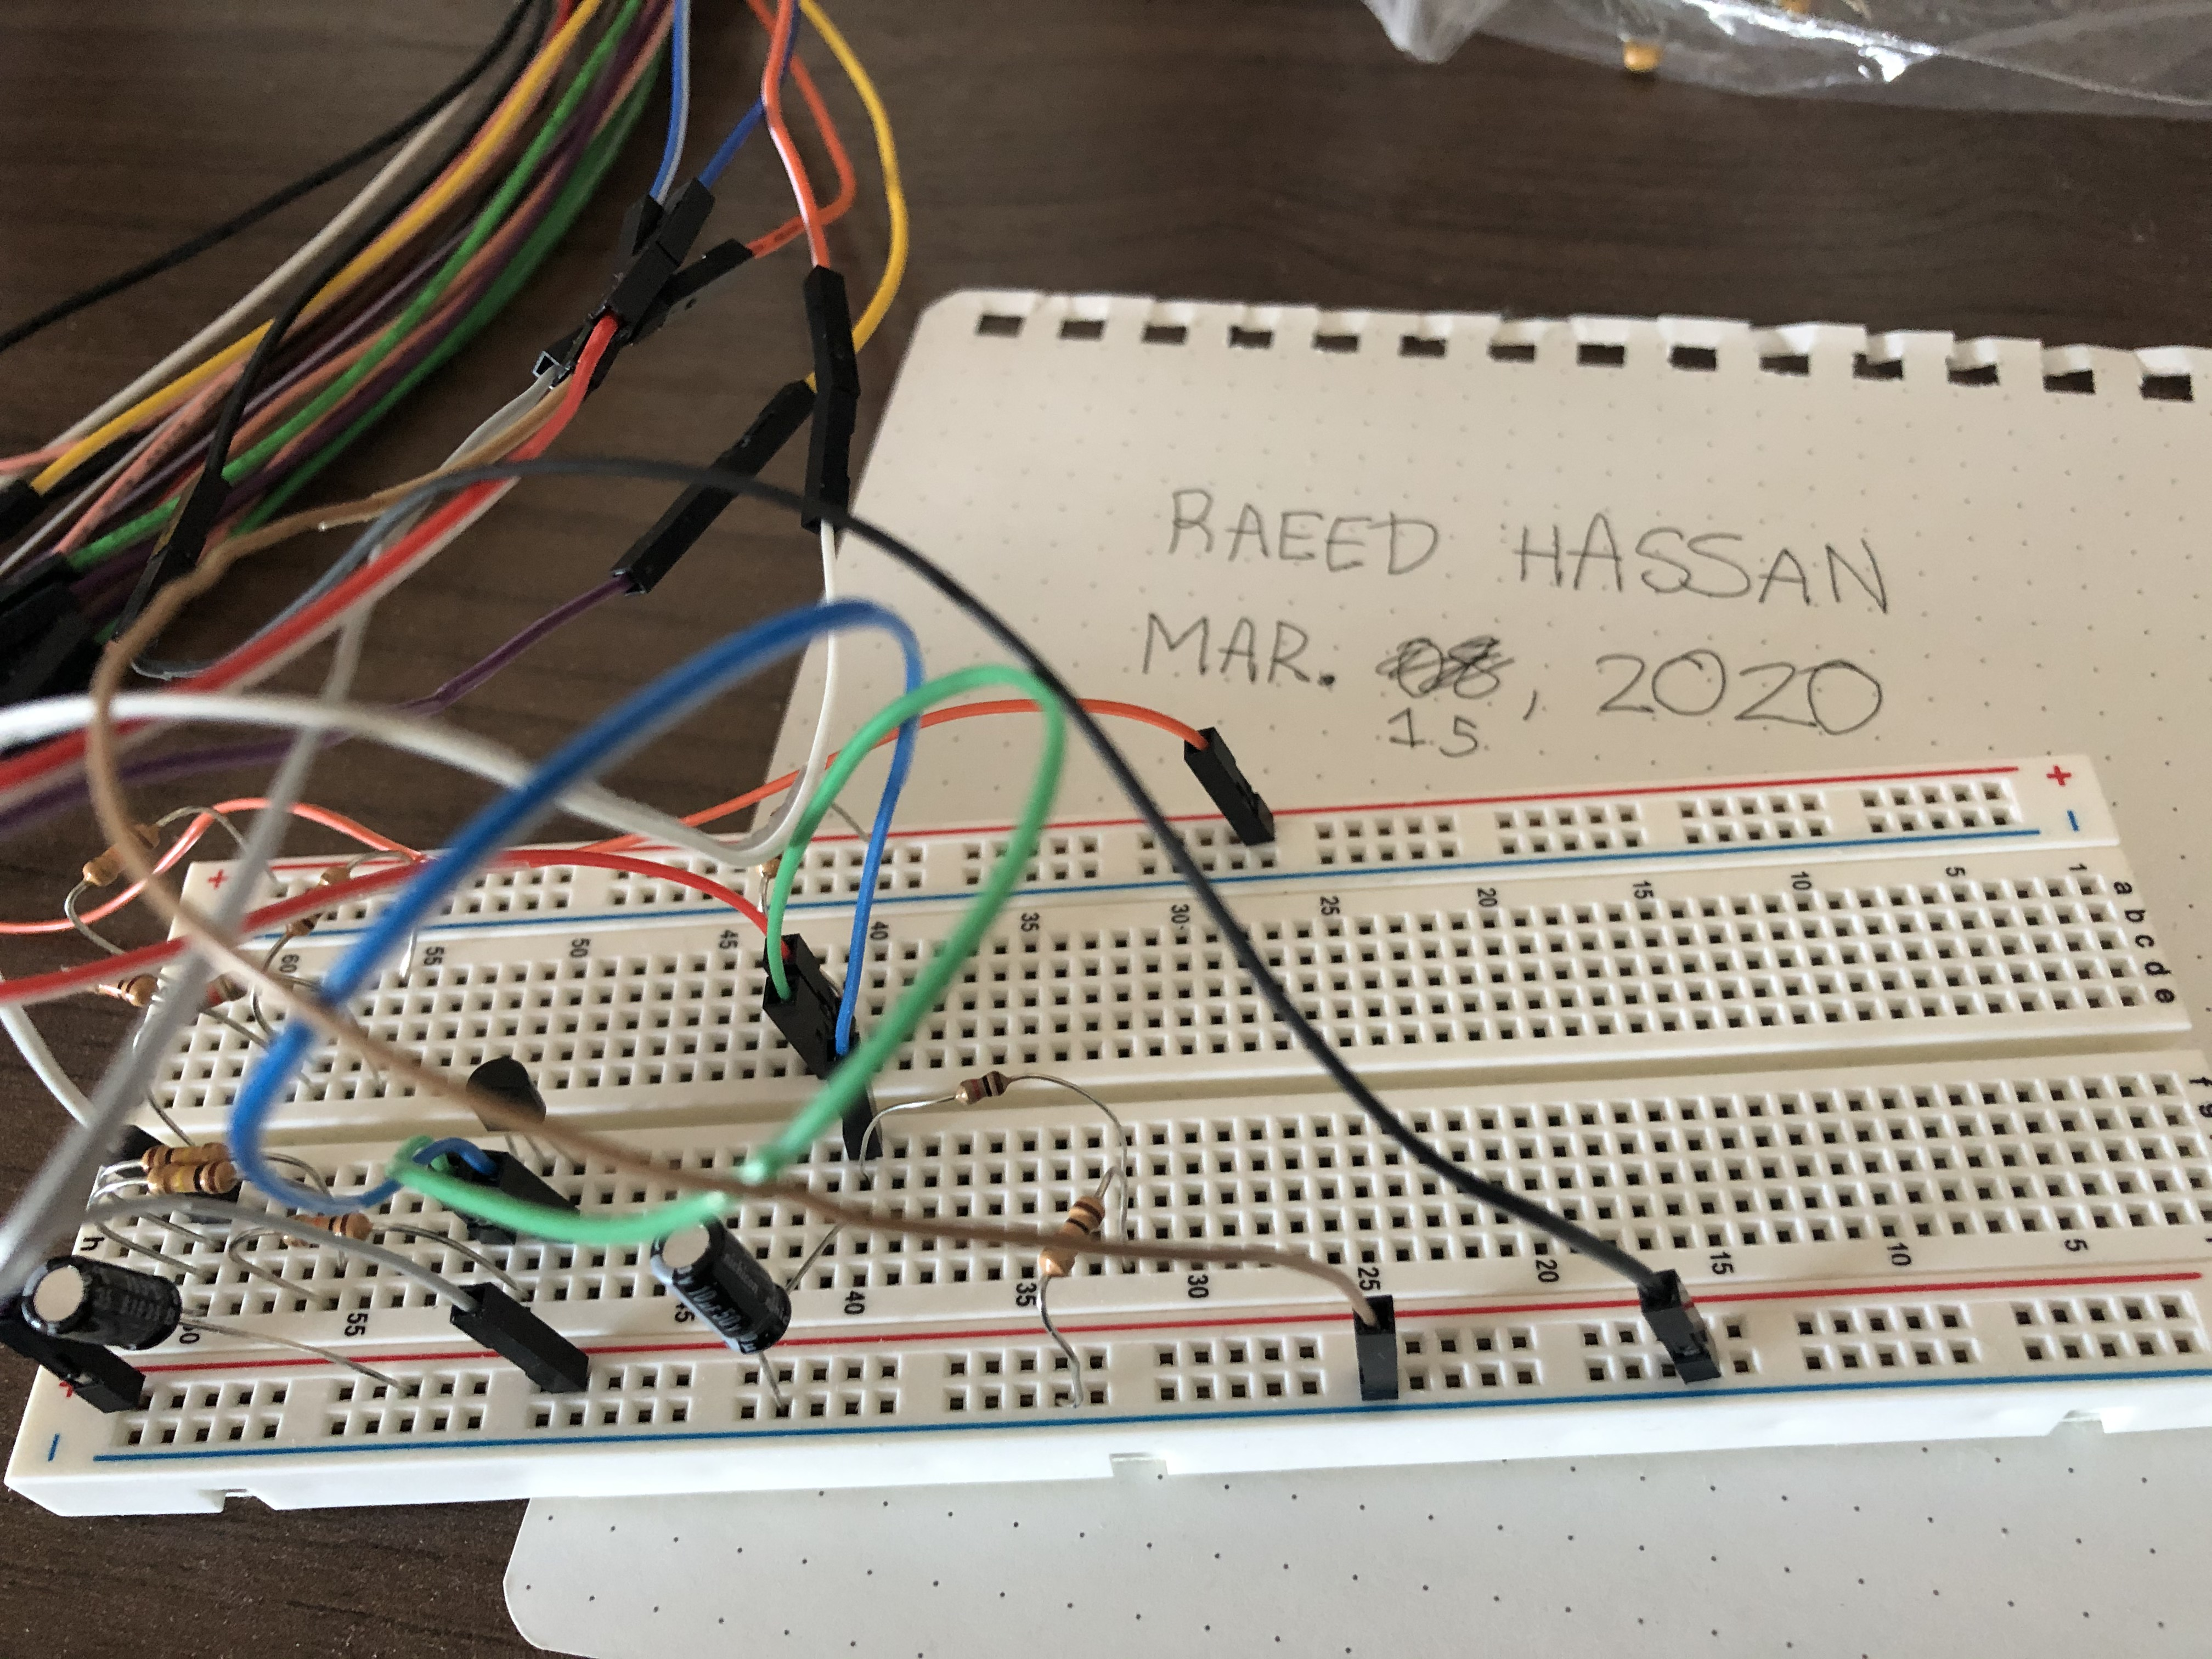
\includegraphics[width=\linewidth]{images/Circuit.png}
    \end{center}
    \item Measurements
    \begin{enumerate}
        \item For the NPN, the circuit had a resistor connected to the wave generator at both the base and the collector. The emitter was connected to ground. To measure $v_{CE}$ and $v_{BE}$, the negative terminal of the scope was connected to the emitter while the positive terminal was connected to the collector or the base. To measure $i_C$ and $i_B$, the voltage drop across the resistor was measured and the current was displayed using a math channel that divided the voltage drop by the resistance of the resistors.
        
        For the PNP, the circuit had a resistor connected to the wave generator at both the base and the emitter. The base was connected to ground. To measure $v_{EC}$ and $v_{BC}$, the negative terminal of the scope was connected to the collector while the positive terminal was connected to the emitter or the base. To measure $i_E$ and $i_B$, the voltage drop across the resistor was measured and the current was displayed using a math channel that divided the voltage drop by the resistance of the resistors. \newpage
        \item 
        Figure 1 shows part a for the NPN at three different values of $i_B$. \\
        \begin{figure}[h!]
            \centering
            \begin{subfigure}[b]{0.31\textwidth}
                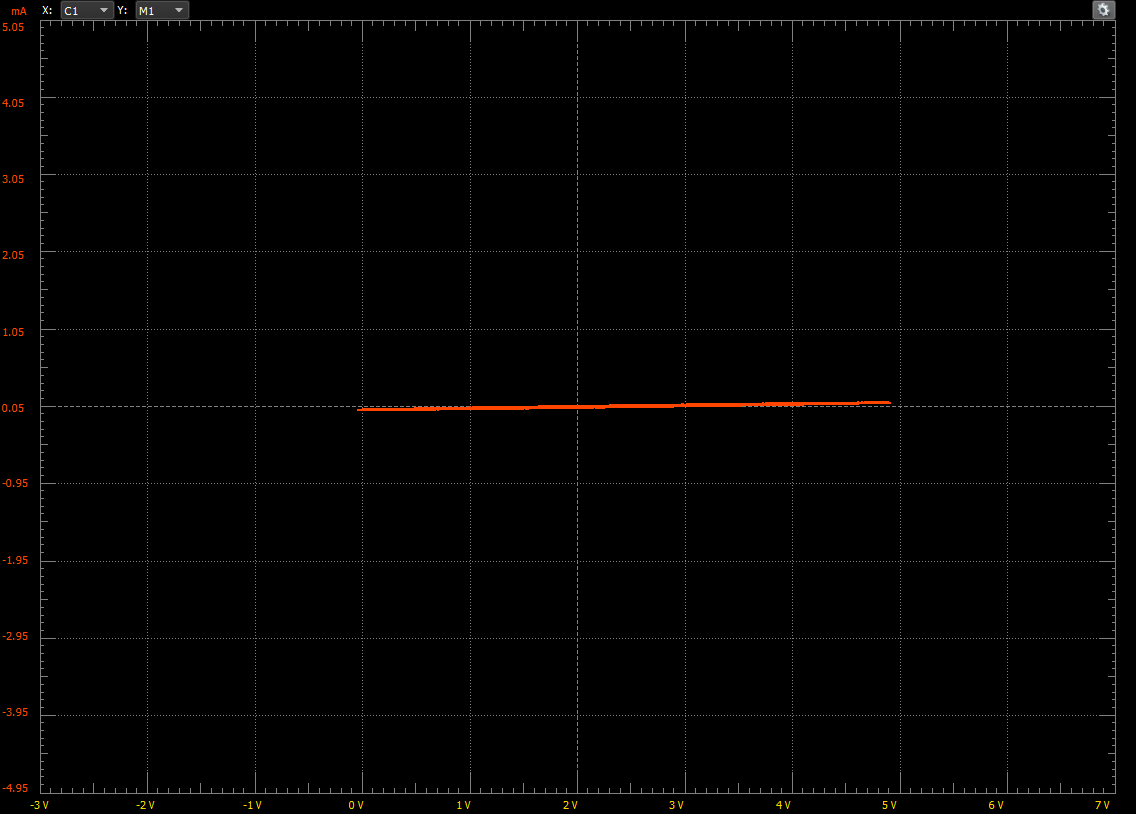
\includegraphics[width=\textwidth]{N1IB0.png}
            \end{subfigure}
            ~
            \begin{subfigure}[b]{0.31\textwidth}
                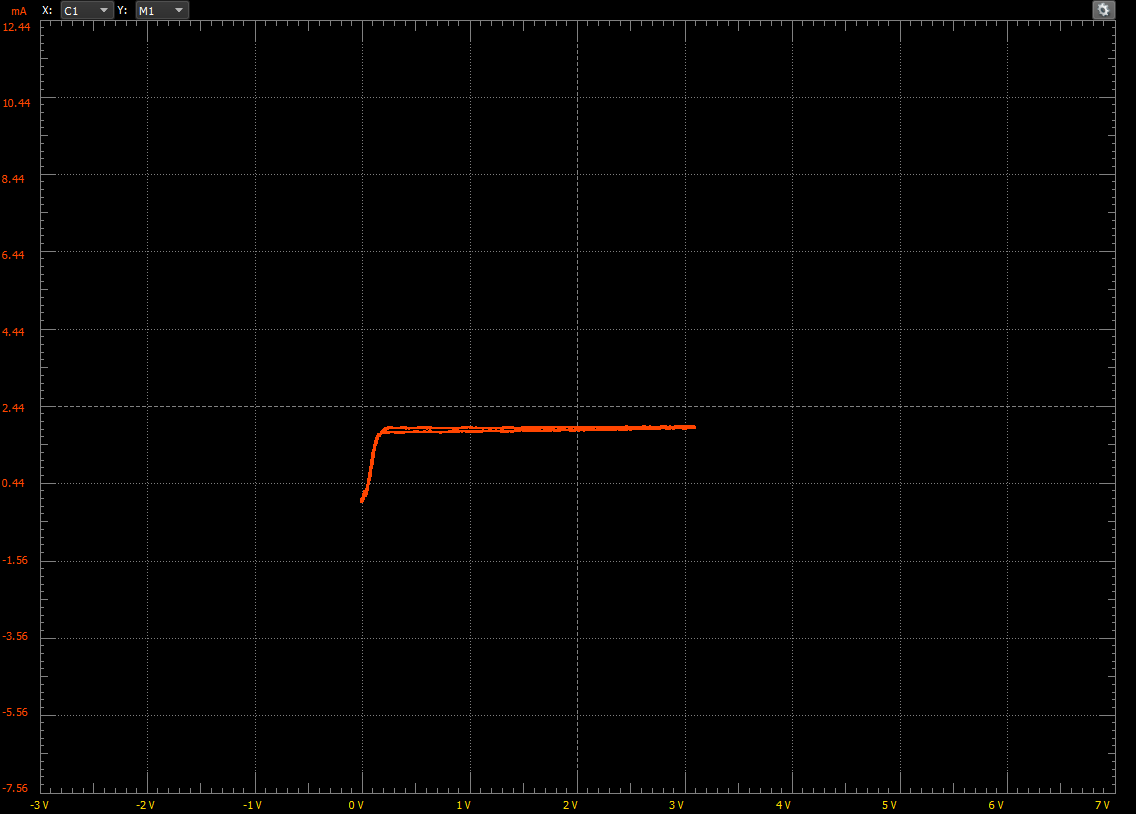
\includegraphics[width=\textwidth]{N1VB650.png}
            \end{subfigure}
            ~
            \begin{subfigure}[b]{0.31\textwidth}
                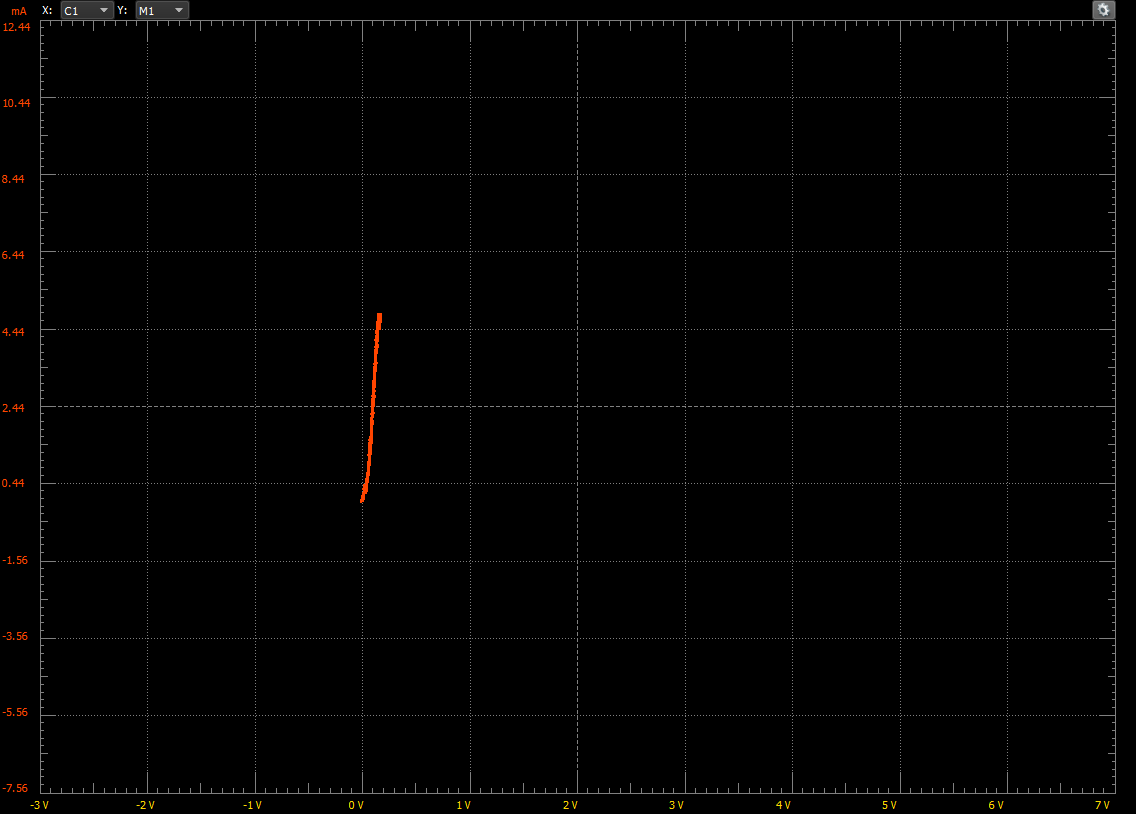
\includegraphics[width=\textwidth]{N1VB700.png}
            \end{subfigure}
            \caption{Part a for three different values of $i_B$}
        \end{figure} \\
        Figure 2 shows $\ln i_C$ as a function of $v_{BE}$ for the NPN in parts b and c. \\
        \begin{figure}[h!]
            \centering
            \begin{subfigure}[b]{0.48\textwidth}
                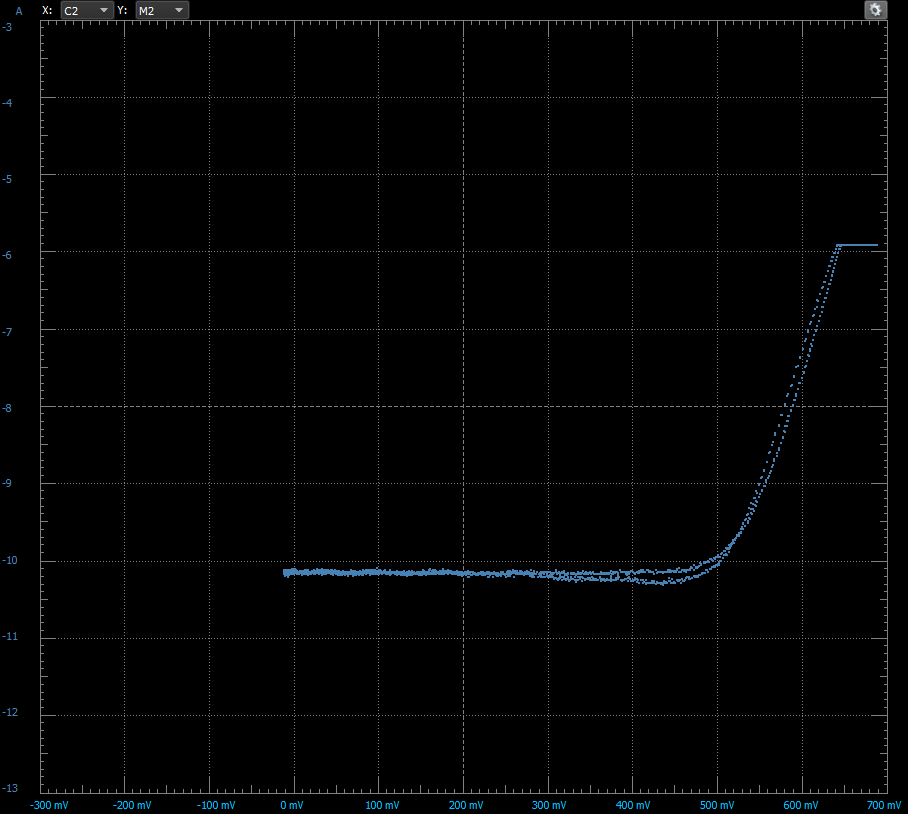
\includegraphics[width=\textwidth]{NBC4.png}
                \caption{$v_{CE} = 4V$}
            \end{subfigure}
            ~
            \begin{subfigure}[b]{0.48\textwidth}
                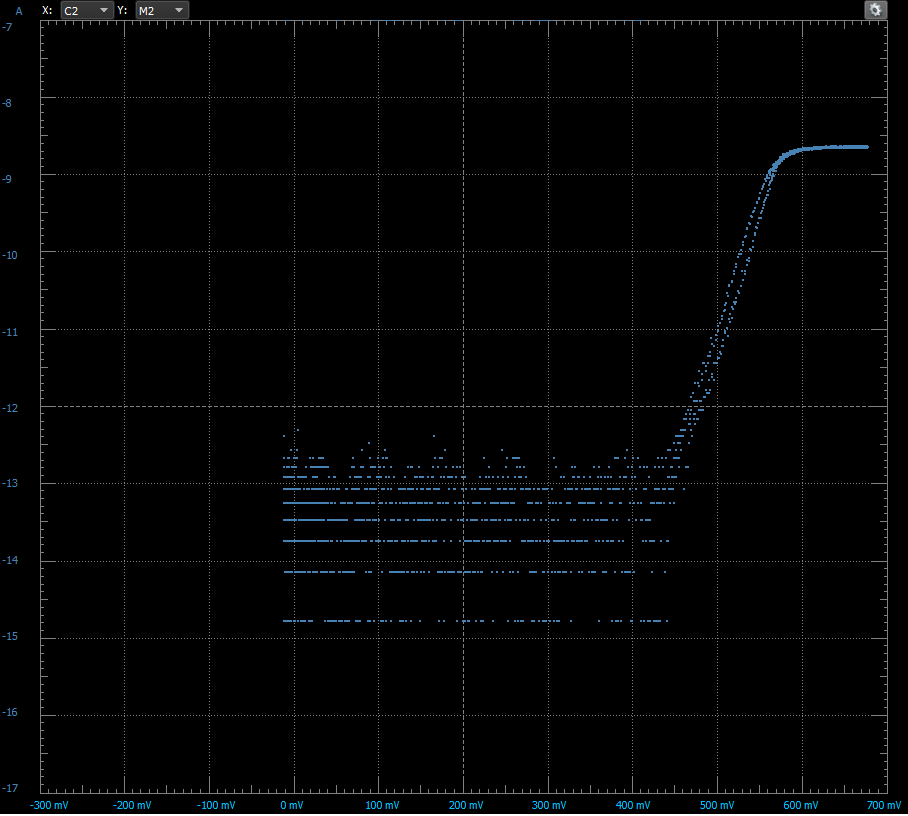
\includegraphics[width=\textwidth]{NCC02.png}
                \caption{$v_{CE} = 0.2V$}
            \end{subfigure}
            \caption{$\ln i_C$ as a function of $v_{BE}$}
        \end{figure} \newpage
        Figure 3 shows $\ln i_B$ as a function of $v_{BE}$ for the NPN in parts b and c. \\
        \begin{figure}[h!]
            \centering
            \begin{subfigure}[b]{0.48\textwidth}
                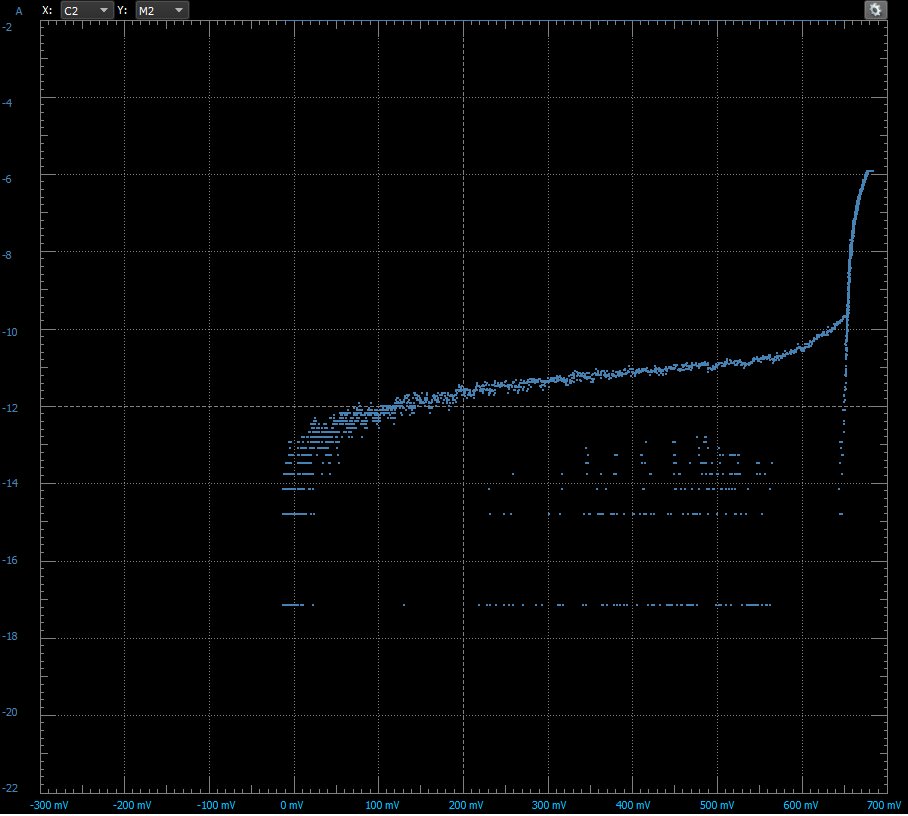
\includegraphics[width=\textwidth]{NBB4.png}
                \caption{$v_{CE} = 4V$}
            \end{subfigure}
            ~
            \begin{subfigure}[b]{0.48\textwidth}
                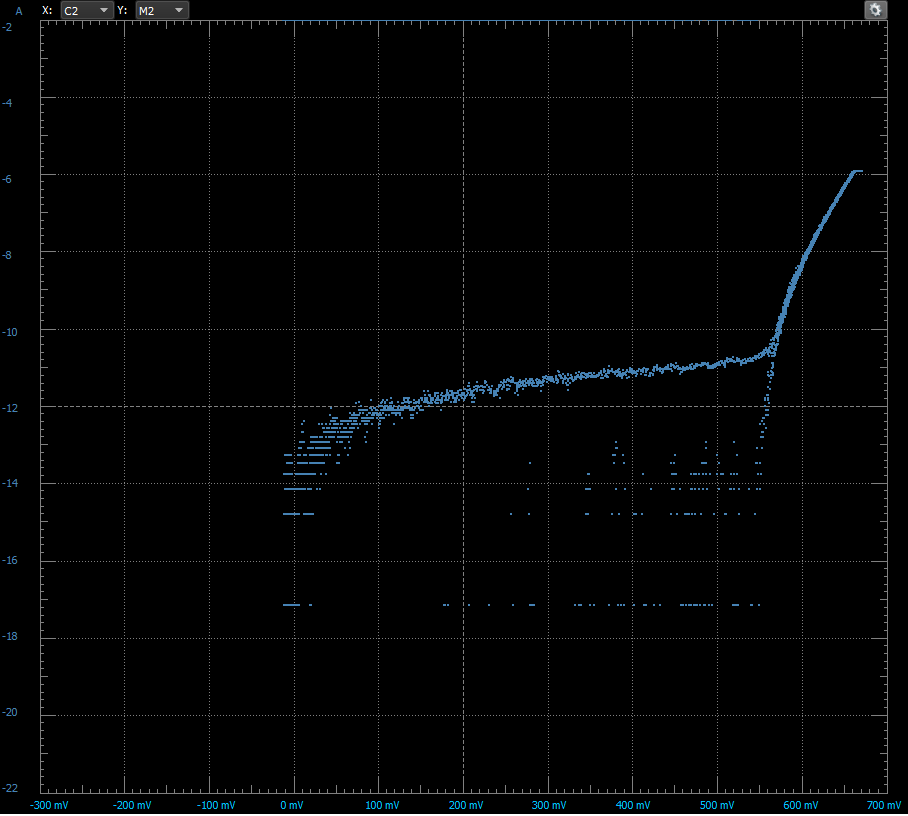
\includegraphics[width=\textwidth]{NCB02.png}
                \caption{$v_{CE} = 0.2V$}
            \end{subfigure}
            \caption{$\ln i_B$ as a function of $v_{BE}$}
        \end{figure} \\
        Figure 4 shows part a for the PNP at three different values of $i_B$. \\
        \begin{figure}[h!]
            \centering
            \begin{subfigure}[b]{0.31\textwidth}
                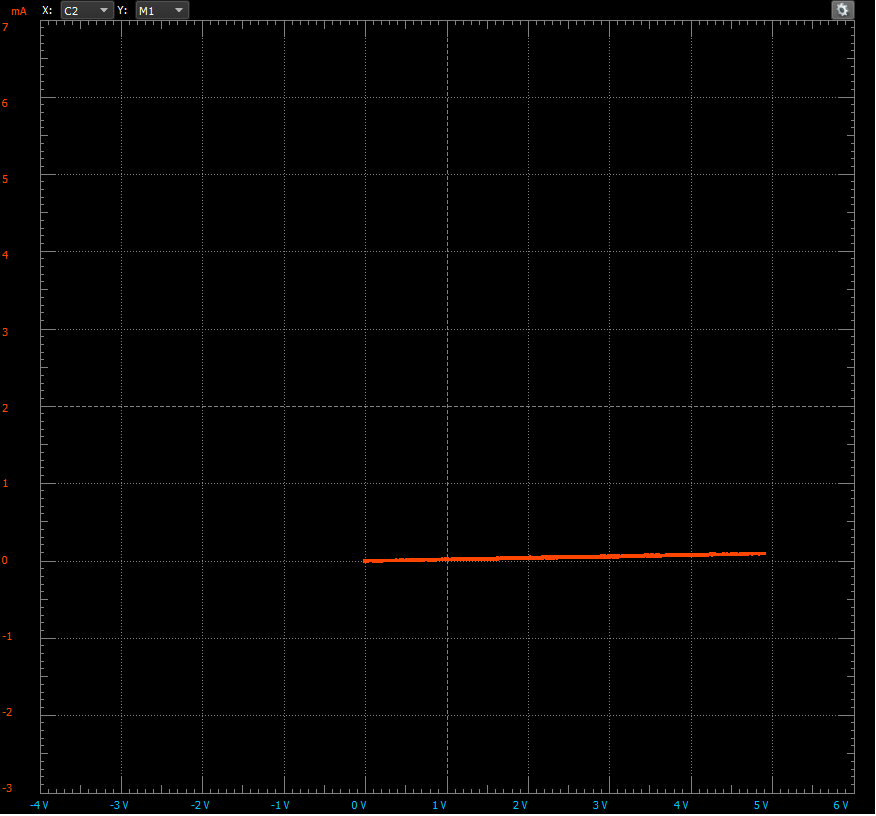
\includegraphics[width=\textwidth]{PAIB0.png}
            \end{subfigure}
            ~
            \begin{subfigure}[b]{0.31\textwidth}
                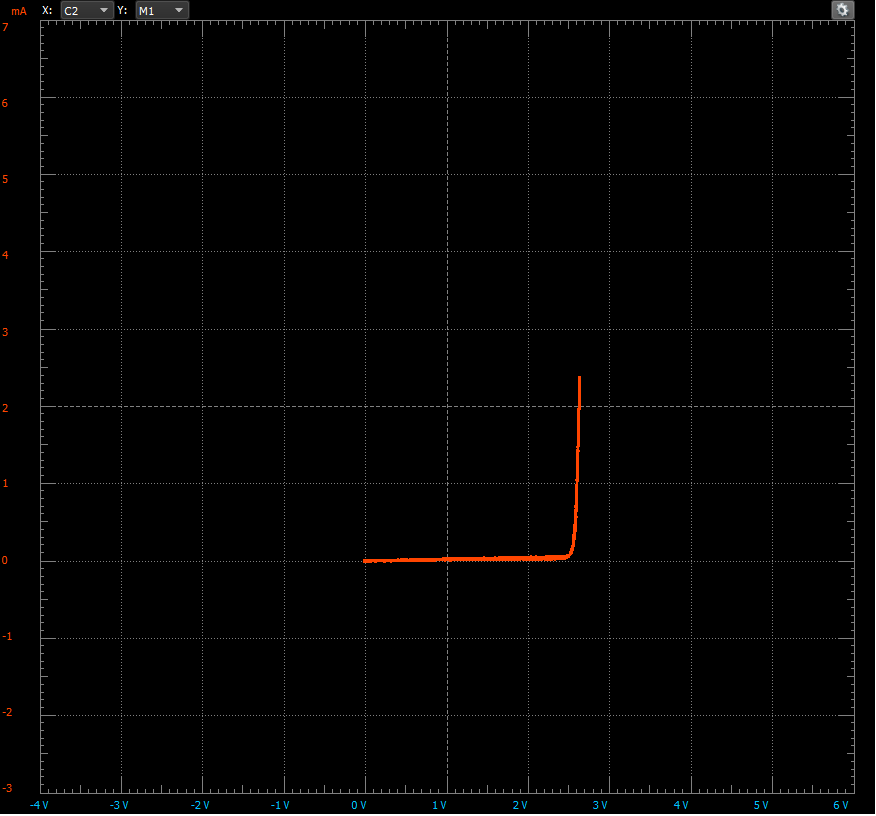
\includegraphics[width=\textwidth]{PAVB3.png}
            \end{subfigure}
            ~
            \begin{subfigure}[b]{0.31\textwidth}
                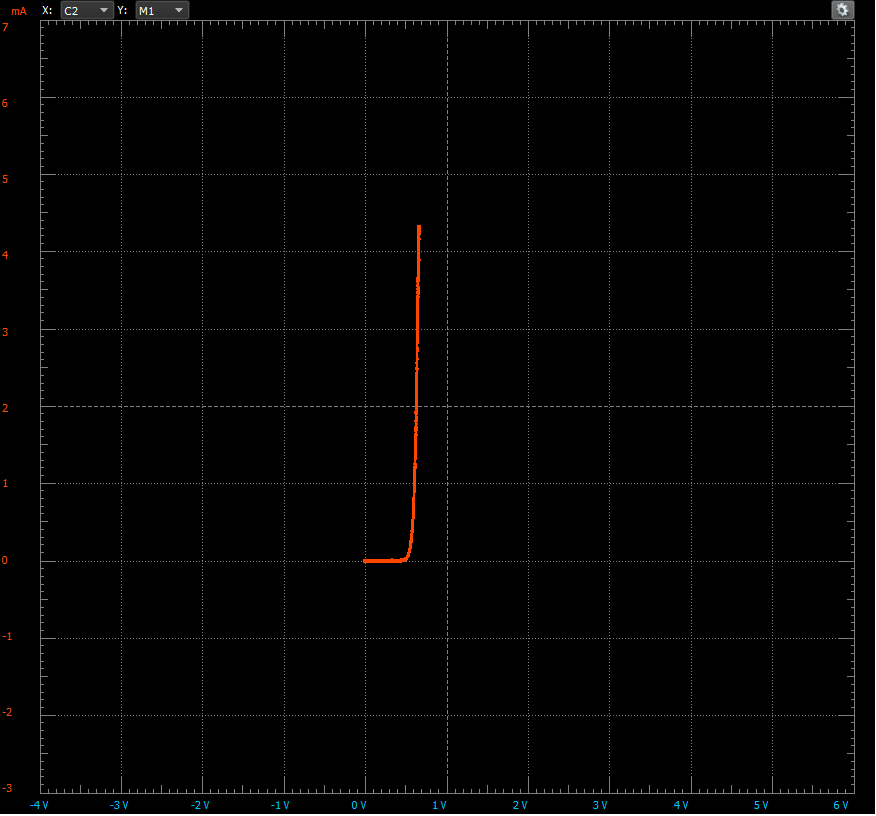
\includegraphics[width=\textwidth]{PAVB5.png}
            \end{subfigure}
            \caption{Part a for three different values of $i_B$}
        \end{figure} \newpage
        Figure 5 shows $\ln i_E$ as a function of $v_{BC}$ for the PNP in parts b and c. \\
        \begin{figure}[h!]
            \centering
            \begin{subfigure}[b]{0.48\textwidth}
                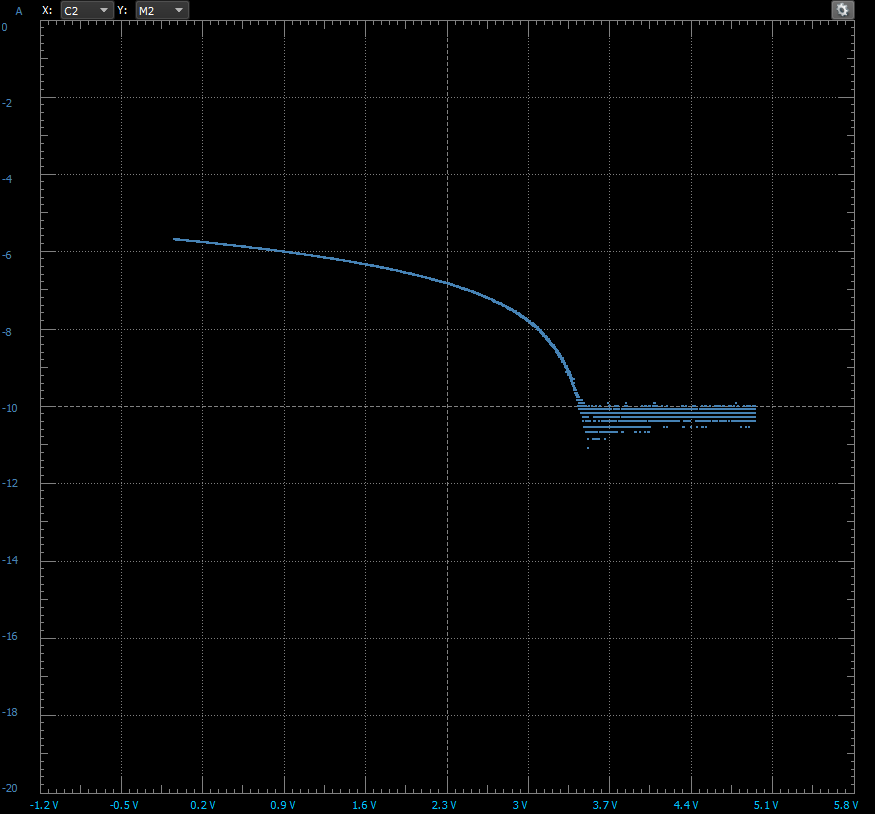
\includegraphics[width=\textwidth]{PBC4.png}
                \caption{$v_{EC} = 4V$}
            \end{subfigure}
            ~
            \begin{subfigure}[b]{0.48\textwidth}
                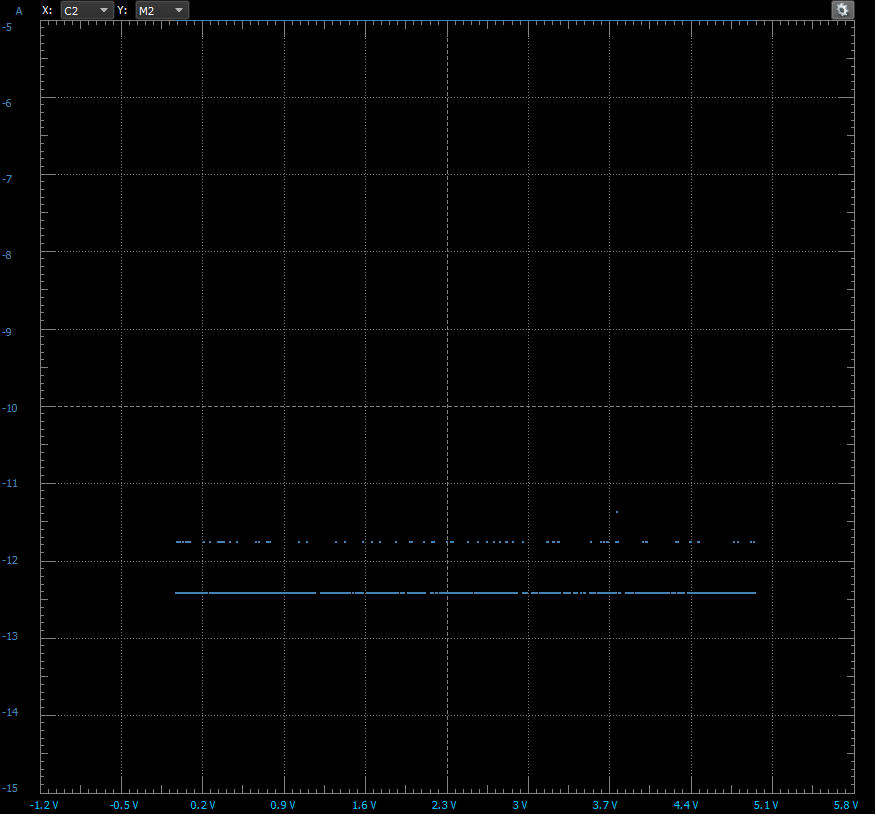
\includegraphics[width=\textwidth]{PCC02.png}
                \caption{$v_{EC} = 0.2V$}
            \end{subfigure}
            \caption{$\ln i_E$ as a function of $v_{BC}$}
        \end{figure} \\
        Figure 6 shows $\ln i_B$ as a function of $v_{BC}$ for the PNP in parts b and c. \\
        \begin{figure}[h!]
            \centering
            \begin{subfigure}[b]{0.48\textwidth}
                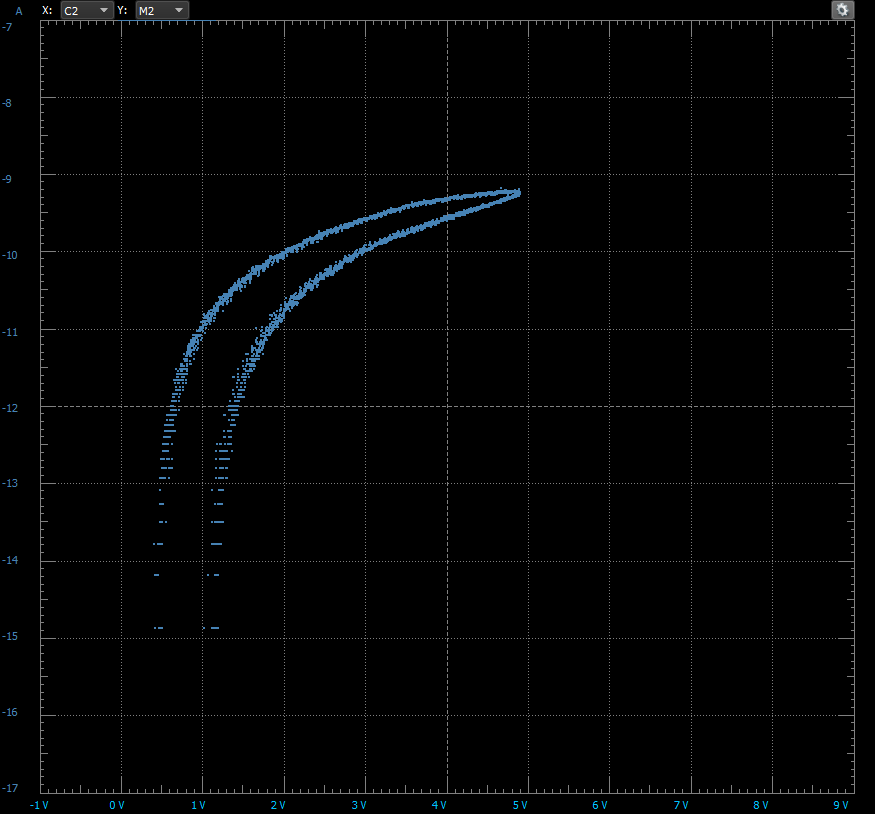
\includegraphics[width=\textwidth]{PBB4.png}
                \caption{$v_{EC} = 4V$}
            \end{subfigure}
            ~
            \begin{subfigure}[b]{0.48\textwidth}
                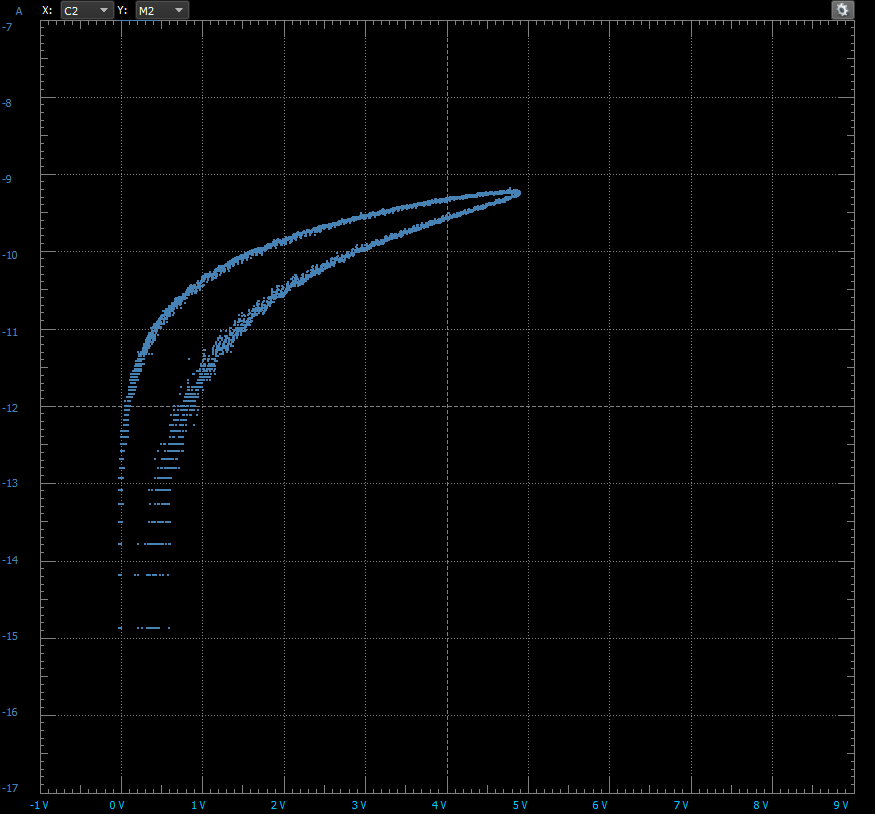
\includegraphics[width=\textwidth]{PCB02.png}
                \caption{$v_{EC} = 0.2V$}
            \end{subfigure}
            \caption{$\ln i_B$ as a function of $v_{BC}$}
        \end{figure} \\
    \end{enumerate}
    To determine the value of $\beta$ for the NPN, you divide the linear region value of $i_C$ found in figure 1 by the value of $i_B$. To determine the value of $\beta$ for the PNP, you take the slope of $i_E$ found in figure 4. To determine the value of $V_{BE(ON)}$ for the NPN, and the value of $V_{BC(ON)}$ for the PNP, you observe the non-zero regions in figures 2 and 5. To determine the value of $V_{CE(sat)}$ for the NPN, and the value of $V_{EC(sat)}$ for the PNP, you observe the the zero regions found in figure 1 and 4.
    \item The marking section of the lab instructions state that no simulations are required for the report.
    \item The shapes of the plots were as expected with little to no discrepancies. Some of the plots did appear to be splitting into different values, however this is because the value of $v_B$ is being changed in those plots, causing the the value of $i_B$ to also change. This causes the graph to shift up and down depending on the value of $i_B$.
    \item For parts b and c, where the value of $v_{CE}$ and $v_{EC}$ had to be set to a certain value, this was not possible using the setup we had. As there had to be a voltage drop across the resistor, the value of $v_C$ or $v_E$ would not be exactly the value that we had for the voltage as the source for the resistor. This likely does not affect performance of the BJTs very much, as except slightly shifting the different modes of operation.
    \end{enumerate}
\end{document}